\documentclass[a4paper,12pt]{article} % тип документа

%  Русский язык
\usepackage[T2A]{fontenc}			% кодировка
\usepackage[utf8]{inputenc}			% кодировка исходного текста
\usepackage[english,russian]{babel}	% локализация и переносы

\usepackage{graphicx}               % импорт изображений
\usepackage{wrapfig}                % обтекаемые изображения
\graphicspath{{pictures/}}          % обращение к подкаталогу с изображениями
\usepackage[14pt]{extsizes}         % для того чтобы задать нестандартный 14-ый размер шрифта
\usepackage{amsfonts}               % буквы с двойными штрихами
\usepackage[warn]{mathtext}         % русский язык в формулах
\usepackage{indentfirst}            % indent first
\usepackage[margin = 25mm]{geometry}% отступы полей
\usepackage{amsmath}                % можно выводить фигурные скобочки -- делать системы уравнений
\usepackage[table,xcdraw]{xcolor}   % таблицы
\usepackage{amsmath,amsfonts,amssymb,amsthm,mathtools} % Математика
\usepackage{wasysym}                % ???
\usepackage{upgreek}                % ???  
\usepackage{caption}
\captionsetup{labelsep=period}
\usepackage{gensymb} % degree symbol

\begin{document}
	\begin{center}
		
		\normalsize{Федеральное государственное автономное образовательное учреждение высшего образования}
		
		\textbf{НАЦИОНАЛЬНЫЙ ИССЛЕДОВАТЕЛЬСКИЙ УНИВЕРСИТЕТ \\ <<МОСКОВСКИЙ ФИЗИКО-ТЕХНИЧЕСКИЙ ИНСТИТУТ>>}
		\vspace{13ex}
		
		\textbf{Лабораторная работа 2.2.1 \\ <<Исследование взаимной диффузии газов>> }
		\vspace{40ex}
		
		\normalsize{Овсянников Михаил Александрович \\ студент группы Б01-001\\ 1 курс ФРКТ\\}
	\end{center}
	
	\vfill 
	
	\begin{center}
		г. Долгопрудный\\ 
		2021 г.
	\end{center}
	
	\thispagestyle{empty} % выключаем отображение номера для этой страницы
	
	\newpage
	
	\textbf{Цель работы:} : 1) регистрация зависимости концентрации гелия в воздухе от времени с помощью датчиков теплопроводности при разных начальных давлениях смеси газов; 2) определение коэффициента диффузии по результатам измерений.
	\\
	\\
\indent	\textbf{В работе используются:}  измерительная установка; форвакуумный насос; баллон с газом (гелий); манометр; источник питания; магазин сопротивлений; гальванометр; секундомер.

\section*{Теоретические сведения}
\indent Диффузией называется самопроизвольное перемешивание молекул, происходящее вследствие их теплового движения. В жидкости диффузия происходит быстрее, чем в твердых телах, а в газах — быстрее, чем в жидкостях. В тех случаях, когда изучается перемешивание молекул одного сорта, говорят о самодиффузии, а если перемешиваются разные молекулы — о взаимной (или концентрационной) диффузии.
	
	
Для исследования взаимной диффузии газов и определения коэффициента диффузии используется установка, изображенная на рис. 1. Два сосуда с объемами $V_{1}$ и $V_{2}$ соединены трубкой длины $l$ и сечения $S$. Сосуды заполнены смесью двух газов при одинаковом давлении, но с различной концентрацией компонентов. Вследствие взаимной диффузии концентрации каждого из компонентов в обоих сосудах с течением времени выравниваются.


Рассмотрим процесс выравнивания концентрации. Пусть концентрации одного из компонентов смеси в сосудах $V_{1}$ и $V_{2}$ равны $n_{1}$ и $n_{2}$. Плотность диффузионного потока любого компонента (т. е. количество вещества, проходящее в единицу времени через единичную поверхность) определяется законом Фика:


\begin{equation}
	j = -D \frac{\partial n}{\partial x}
\end{equation}

где $D$ - коэффициент взаимной диффузии газов, а $j$ - плотность потока частиц. В наших условиях решение задачи упрощается благодаря тому, что: а) объем соединительной трубки мал по сравнению с объемами сосудов, б) концентрацию газов внутри каждого сосуда можно считать постоянной по всему объему. Диффузионный поток в любом сечении трубки одинаков. Поэтому $J = -DS(\partial n/\partial x)$ не меняется вдоль трубки. Следовательно,


\begin{equation}
	J = - DS\frac{n_{1} - n_{2}}{l}.
\end{equation}

\newpage

\begin{figure}[h!]
	\centering
	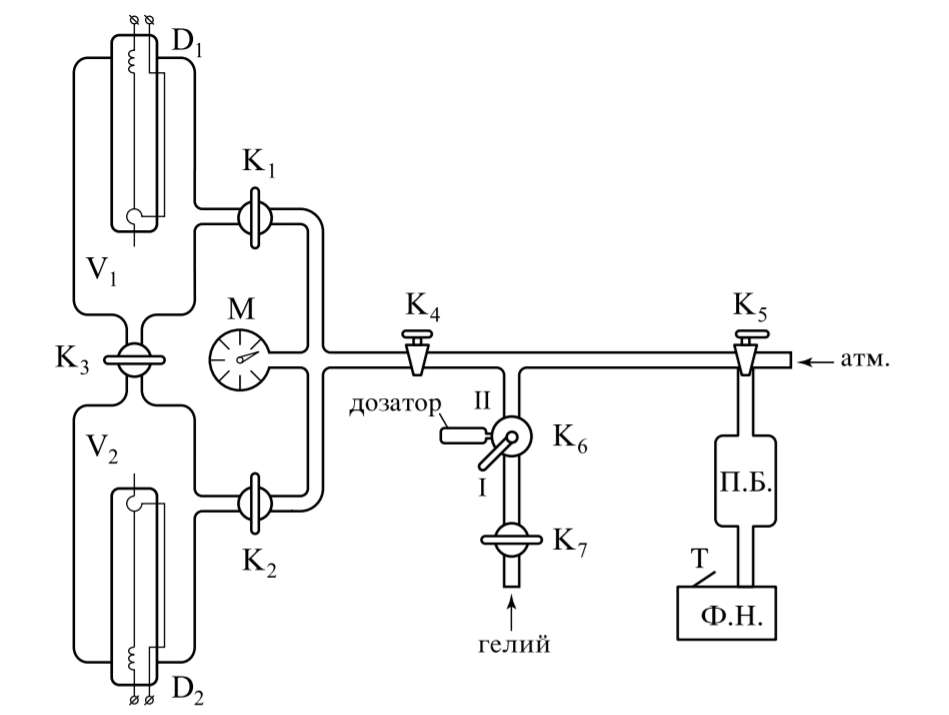
\includegraphics[scale=0.8]{Pictures/Рис1.png}
	\caption{Установка для исследования взаимной диффузии газов}
\end{figure}

Обозначим через $\Delta n_{1}$ и $\Delta n_{2}$ изменения концентрации в объемах $V_{1}$ и $V_{2}$ за время $\Delta t$. Тогда $V_{1} \Delta n_{1}$ равно изменению количества компонента в объеме $V_{1}$, а $V_{2}\Delta n_{2}$ — изменению количества этого компонента в $V_{2}$. Из закона сохранения вещества следует, что $V_{1}n_{1} + V_{2}n_{2} = $ const, откуда $V_{1}\Delta n_{1} = -V_{2}\Delta n_{2}$. Эти изменения происходят вследствие диффузии, поэтому


\begin{equation}
	V_{1}\Delta n_{1} = -V_{2}\Delta n_{2} = J\Delta t = -DS \frac{n_{1} - n_{2}}{l}\Delta t.
\end{equation}


\noindent Деля это равенство на $\Delta t$, получим


\begin{equation}
	V_{1}\frac{dn_{1}}{dt} = -DS\frac{n_{1} - n_{2}}{l}, \hspace{10mm} V_{2}\frac{dn_{2}}{dt} = DS\frac{n_{1} - n_{2}}{l}.
\end{equation}


\noindent Разделив первое из этих уравнений на $V_{1}$, а второе на $V_{2}$ и вычтя эти равенства друг из друга, найдем


\begin{equation}
	\frac{dn_{1}}{dt} - \frac{dn_{2}}{dt} = -\frac{n_{1} - n_{2}}{l}DS\left(\frac{1}{V_{1}} + \frac{1}{V_{2}}\right).
\end{equation}


\noindent Введем новую переменную $n_{1} - n_{2}$, после чего уравнение легко интегрируется:


\begin{equation}
	n_{1} - n_{2} = (n_{1} - n_{2})_{0}e^{-t/\tau},
\end{equation}


\noindent где $(n_{1} - n_{2})_{0}$ — разность концентраций в начальный момент времени,


\begin{equation}
	\tau = \frac{V_{1}V_{2}}{V_{1} + V_{2}}\frac{l}{SD}.
\end{equation}


\noindent Формула (6) показывает, что разность концентраций убывает по экспоненциальному закону, и тем быстрее, чем меньше $\tau$ (постоянная времени процесса). Величина $\tau$ определяется геометрическими размерами установки $(l, S, V_{1}, V_{2})$ и величиной коэффициента диффузии $D$.


Для измерения концентраций в данной установке применяются датчики теплопроводности D$_{1}$ и D$_{2}$ (см. рис. 1) и используется зависимость теплопроводности газовой смеси от ее состава. Тонкая проволочка радиуса $r_{\text{пр}}$, протянутая вдоль оси стеклянного цилиндра радиуса $R_{\text{ц}}$, нагревается током. Тепло от проволочки к стенке цилиндра переходит главным образом вследствие теплопроводности газа, находящегося внутри цилиндра. Количество тепла, передающееся стенке в единицу времени, получим:


\begin{equation}
	Q = \varkappa\frac{2\pi L}{\ln{(R_{\text{ц}}/r_{\text{пр}})}}(T_{1} - T_{2}),
\end{equation}



\noindent где $\varkappa$ — теплопроводность, $L$ — длина нити, $T_{1}, T_{2}$ — температуры проволочки и стенки. При заданном режиме нагревания ($Q = $ const) температура проволочки и соответственно ее сопротивление определяются теплопроводностью газа и, следовательно, его составом.



Для измерения разности концентраций газов используется мостовая схема (рис. 2). Здесь D$_{1}$ и D$_{2}$ — датчики теплопроводности, расположенные в сосудах $V_{1}$ и $V_{2}$. Сопротивления $R_{1}, R_{2}$ и $R$ служат для установки прибора на нуль (балансировка моста). В одну из диагоналей моста включен гальванометр, к другой подключается небольшое постоянное напряжение. Мост балансируется при заполнении сосудов (и датчиков) одной и той же смесью. При заполнении сосудов смесями различного состава возникает «разбаланс» моста, зависящий от разности концентраций.


Зависимость теплопроводности смеси газов от ее состава, вообще говоря, довольно сложна. Однако при достаточно малых изменениях концентраций можно ожидать, что величина тока, проходящего через гальванометр G , будет пропорциональна разности концентраций (первый член разложения функции в ряд Тейлора). Эксперименты показывают, что при разности концентраций, равной 15\%, поправка к линейному закону не превышает 0,5\%, что для наших целей вполне достаточно.

\begin{wrapfigure}{R}{0.35\textwidth}
	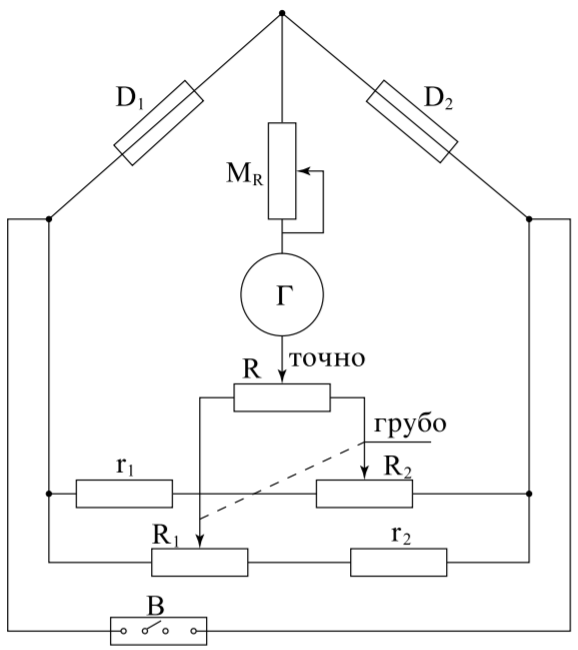
\includegraphics[width=0.35\textwidth]{Pictures/Рис2.png}
	\caption*{\footnotesize{Рис. 2. Мостовая схема с датчиками теплопроводности для измерения разности концентраций газов}}
\end{wrapfigure}


В процессе диффузии разность концентраций убывает по закону (6). По тому же закону изменяются во времени показания гальванометра (например, в делениях шкалы), т. е.



\begin{equation}
	N = N_{0}e^{-t/\tau},
\end{equation}


\noindent где $N_{0}$ — показание в начальный момент времени.


\vspace{5mm}
Отметим некоторые особенности методики, примененной в данной работе.


1. Для устранения тепловой конвекции датчик выполнен в виде длинной стеклянной трубки, внутри которой натянута нагреваемая током платиновая нить. Внутренняя полость датчика сообщается с объемом камеры через специально сделанные отверстия. Размер отверстий и объем датчика таковы, что скорость диффузии газов из объема сосуда в полость датчика значительно больше скорости диффузии из одного объема в другой. Таким образом, состав газа в датчике практически совпадает с составом газа в объеме.


2. В силу неполного обмена энергией между молекулами газа и поверхностью нити её температура несколько выше, чем температура прилегающих слоев газа — на ее поверхности возникает температурный скачок. Величина температурного скачка зависит от давления. Вследствие этого, а также потому, что датчики не абсолютно идентичны, баланс моста несколько зависит от давления. Для повышения точности опытов рекомендуется балансировать мост, заполнив установку воздухом при давлении, близком к рабочему.

\newpage
\section*{Экспериментальная установка}
Общий вид конструкции установки приведен на рис. 1. Схема электрических соединений показана на рис. 2. На рис. 3 изображена конструкция многоходового крана К$_{6}$.


\begin{wrapfigure}{R}{0.35\textwidth}
	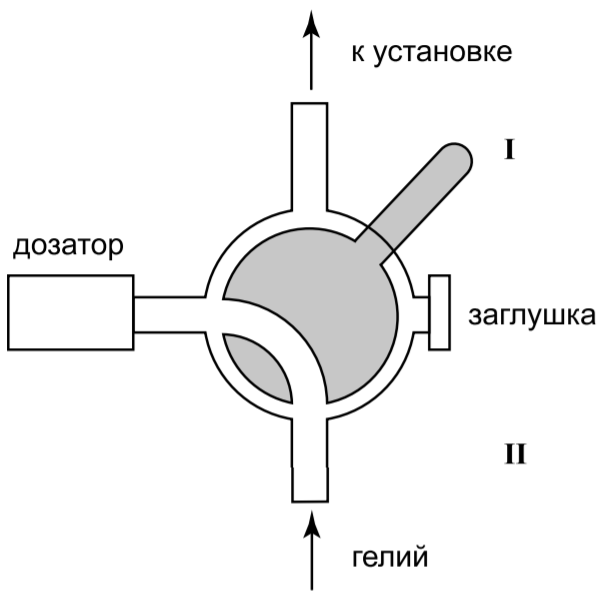
\includegraphics[width=0.35\textwidth]{Pictures/Рис3.png}
	\caption*{\footnotesize{Рис. 3. Кран K$_{6}$}}
\end{wrapfigure}


Установка состоит из двух сосудов $V_{1}$ и $V_{2}$ соединенных краном K$_{3}$, форвакуумного насоса Ф.Н. с выключателем Т, манометра M и системы напуска гелия, включающей в себя краны K$_{6}$ и K$_{7}$. Кран K$_{5}$ позволяет соединять форвакуумный насос либо с установкой, либо с атмосферой. Между форвакуумным насосом и краном K$_{5}$ вставлен предохранительный баллон П.Б., защищающий кран K$_{5}$ и установку при неправильной эксплуатации ее от попадания форвакуумного масла из насоса Ф.Н. Сосуды $V_{1}$ и $V_{2}$ и порознь и вместе можно соединять как с системой напуска гелия, так и с форвакуумным насосом. Для этого служат краны K$_{1}$, K$_{2}$, K$_{4}$ и K$_{5}$. Манометр M регистрирует давление газа, до которого заполняют тот или другой сосуды.


Давление гелия в трубопроводе больше атмосферного. Это необходимо для того, чтобы из-за возможных неплотностей в трубопроводе гелий оставался бы в нем без примесей воздуха. А система напуска гелия, особенно многоходовой кран K$_{6}$, как правило, имеет утечки. Для сохранения гелия, а также для уменьшения неконтролированного попадания гелия в установку (по протечкам в кране K$_{6}$) между трубопроводом подачи гелия и краном К$_{6}$ поставлен металлический кран K$_{7}$. Его открывают только на время непосредственного заполнения установки гелием. Все остальное время он закрыт.


В силу того, что в сосуд требуется подавать малое давление гелия, между кранами K$_{7}$ и K$_{4}$ стоит кран K$_{6}$, снабженный дозатором. Дозатор — это маленький объем, который заполняют до давления гелия в трубопроводе, а затем уже эту порцию гелия с помощью крана K$_{6}$ впускают в установку. Подробно разрез крана K$_{6}$ приведен на рис. 3. На этом рисунке показано соединение трубопровода гелия с дозатором. Рычажок Р (рис. 1 и 3), показанный пунктиром, находится в квадранте I. Для подачи гелия из дозатора в установку необходимо рычажок Р перевести из квадранта I в квадрант II. Если при этом окажется, что однократной подачи недостаточно, то процедуру надо повторить. Если же окажется, что гелия напущено больше необходимого, излишки можно откачать форвакуумным насосом. Устройство крана K$_{6}$ не на всех установках одинаково, но на всех установках одинаков его принцип — гелий в установку подается малыми порциями.


Кран K$_{4}$ обладает повышенной вакуумоплотностью. Как отмечалось выше, кран K$_{6}$ такой плотностью не обладает. Поэтому после заполнения сосудов $V_{1}$ и $V_{2}$ рабочей смесью кран K$_{4}$ надо обязательно закрыть, чтобы в рабочей части установки давление в процессе измерений сохранялось постоянным.


На рис. 2 приведена схема электрического соединения. D$_{1}$ и D$_{2}$ — сопротивления проволок датчиков парциального давления, которые составляют одно плечо моста. Второе плечо моста составляют сопротивления $r_{1}, R_{1}$ и $r_{2}, R_{2}$. $r_{1} \ll R_{1}$, $r_{2} \ll R_{2}$, $R_{1}$ и $R_{2}$ спаренные, их подвижные контакты находятся на общей оси. Оба они используются для грубой регулировки моста. Точная балансировка моста выполняется потенциометром $R$. Последовательно с гальванометром Г, стоящим в диагонали моста, поставлен магазин сопротивлений $M_{R}$. Когда мост балансируют, магазин сопротивлений выводят на ноль. В процессе же составления рабочей смеси в сосудах $V_{1}$ и $V_{2}$ мост разбалансирован. Чтобы не сжечь при этом гальванометр, магазин $M_{R}$ ставят на максимальное сопротивление.


\section*{Ход работы}
\begin{enumerate}
	\item Ознакомимся с установкой.
	
	\item Включим питание электрической схемы установки рубильником B (рис. 2). Откроем краны K$_{1}$, K$_{2}$, K$_{3}$.
	
	\item Очистим установку от всех газов, которые в ней есть. Для этого откроем кран K$_{4}$. Включим форвакуумный насос (Ф.Н.) выключателем Т, находящемся на насосе, и соединим насос с установкой, повернув ручку крана K$_{5}$ длинным концом рукоятки влево (на установку). Откачаем установку до давления $\thicksim$0,1 торр, что достигается непрерывной работой насоса в течение 3–5 минут. Для прекращения откачки ручку крана K$_{5}$ поставим длинным концом вверх. 
	
	\item Затем в установку напустим воздух до рабочего давления (вначале $P = $ 40 торр), чтобы сбалансировать мост на рабочем давлении. Для этого рукоятку крана K$_{5}$ повернем из положения вправо в положение влево. Повторяем эту операцию несколько раз, пока не будет достигнуто нужное давление. Если окажется, что воздуха мы напустили слишком много, излишки его откачиваем тем же насосом.
	
	
	Сбалансируем мост. Балансировку моста начинаем при сопротивлении магазина сопротивлений $M_{R} \thicksim 10^{5}$ Ом, добиваясь нулевых показаний гальванометра Г вначале с помощью ручки «грубо» (рис. 2) постепенно уменьшая сопротивление магазина до 0, а затем с помощью ручки «точно». Когда баланс достигнут, переключатели моста установить на максимум. Это необходимо сделать для того, чтобы в процессе последующих действий не сжечь гальванометр.
	
	\item Заполним установку рабочей смесью: в сосуде $V_{2}$ воздухом, а в сосуде $V_{1}$ - смесь воздуха с гелием. Заполнение производим в следующем порядке:
	
	а) Откачиваем установку до $\thicksim$ 0,1 торр.
	
	
	б) Закрываем краны K$_{2}$ и K$_{3}$, прежде убедившись в том, что краны K$_{1}$ и K$_{4}$ открыты.
	
	
	в) Заполняем объем $V_{1}$ гелием до давления 0,2$P_{\text{рабочее}}$, т. е. 4 торр. Давление гелия в трубопроводе немного выше атмосферного и, следовательно, много больше требуемых 4 торр. Поэтому соединять напрямую полость установки с трубопроводом гелия нельзя. Гелием наполняем сначала дозатор, а уже потом (см. рис. 3) дозатор соединяем с полостью установки. Эту операцию проводим с помощью крана K$_{6}$, поворачивая его рукоятку из положения I в положение II и обратно до тех пор, пока не будет достигнуто нужное давление. Если давление гелия оказалось слишком большим, его излишки откачиваем насосом. После заполнения ёмкости $V_{1}$ гелием кран K$_{1}$ закрываем, а из патрубков установки откачиваем оставшийся гелий до 0,1 торр.
	
	
	г) Открываем кран K$_{2}$ и с помощью крана K$_{5}$ заполняем объём $V_{2}$ воздухом до давления 1,75$P_{\text{рабочее}}$. После этого закрываем кран K$_{4}$. Это необходимо сделать потому, что его герметичность выше, чем у остальных соединений справа от него, и особенно у крана K$_{6}$.
	
	
	д) Уравняем давление в объемах $V_{1}$ и $V_{2}$, открыв кран K$_{1}$ при уже открытом кране K$_{2}$. Пока идёт выравнивание давлений и температур, подготовим измерительную схему к работе. Для этого, постепенно уменьшая величину сопротивления $M_{R}$, добьемся, чтобы показания вольтметра были $\thicksim 0 $ мВ.
	
	
	\item Приступаем к измерениям. Откроем кран K$_{3}$ и будем отмечать, как изменяются показания вольтметра с течением времени (таблица 1). Процесс измерений продолжаем до тех пор, пока разность концентраций не упадет на 30–50\%.
	
	
	\item Продолжаем аналогичные измерения (п. 3–6) при различных 5 (в сумме) значениях $P_{\text{рабочее}}$: 40, 60, 90, 140, 250 торр (таблицы 1-5).

	
	
\begin{table}[h!]
	\centering
	\begin{tabular}{lllccllllll}
		\cline{1-3} \cline{9-11}
		\multicolumn{3}{|c|}{$P = 40$ торр}                                                          &                      &                      &  &  & \multicolumn{1}{l|}{} & \multicolumn{3}{c|}{$P = $ 60 торр}                                                         \\ \cline{1-3} \cline{9-11} 
		\multicolumn{1}{|c|}{$t$, c}  & \multicolumn{1}{c|}{$U$, мВ} & \multicolumn{1}{c|}{$\ln{U}$} &                      &                      &  &  & \multicolumn{1}{l|}{} & \multicolumn{1}{c|}{$t$, c}  & \multicolumn{1}{c|}{$U$, мВ} & \multicolumn{1}{c|}{$\ln{U}$} \\ \cline{1-3} \cline{9-11} 
		\multicolumn{1}{|l|}{0,000}   & \multicolumn{1}{l|}{23,5184} & \multicolumn{1}{l|}{3,1578}   &                      &                      &  &  & \multicolumn{1}{l|}{} & \multicolumn{1}{l|}{0,000}   & \multicolumn{1}{l|}{19,5711} & \multicolumn{1}{l|}{2,9741}   \\ \cline{1-3} \cline{9-11} 
		\multicolumn{1}{|l|}{25,893}  & \multicolumn{1}{l|}{21,2177} & \multicolumn{1}{l|}{3,0548}   &                      &                      &  &  & \multicolumn{1}{l|}{} & \multicolumn{1}{l|}{30,165}  & \multicolumn{1}{l|}{18,3448} & \multicolumn{1}{l|}{2,9093}   \\ \cline{1-3} \cline{9-11} 
		\multicolumn{1}{|l|}{50,893}  & \multicolumn{1}{l|}{19,5227} & \multicolumn{1}{l|}{2,9716}   &                      &                      &  &  & \multicolumn{1}{l|}{} & \multicolumn{1}{l|}{60,165}  & \multicolumn{1}{l|}{17,3511} & \multicolumn{1}{l|}{2,8537}   \\ \cline{1-3} \cline{9-11} 
		\multicolumn{1}{|l|}{75,893}  & \multicolumn{1}{l|}{17,8510} & \multicolumn{1}{l|}{2,8821}   &                      &                      &  &  & \multicolumn{1}{l|}{} & \multicolumn{1}{l|}{90,165}  & \multicolumn{1}{l|}{16,3083} & \multicolumn{1}{l|}{2,7917}   \\ \cline{1-3} \cline{9-11} 
		\multicolumn{1}{|l|}{100,893} & \multicolumn{1}{l|}{16,4461} & \multicolumn{1}{l|}{2,8001}   &                      &                      &  &  & \multicolumn{1}{l|}{} & \multicolumn{1}{l|}{120,165} & \multicolumn{1}{l|}{15,1540} & \multicolumn{1}{l|}{2,7183}   \\ \cline{1-3} \cline{9-11} 
		\multicolumn{1}{|l|}{127,893} & \multicolumn{1}{l|}{15,7900} & \multicolumn{1}{l|}{2,7594}   &                      &                      &  &  & \multicolumn{1}{l|}{} & \multicolumn{1}{l|}{150,165} & \multicolumn{1}{l|}{14,0296} & \multicolumn{1}{l|}{2,6412}   \\ \cline{1-3} \cline{9-11} 
		\multicolumn{1}{|l|}{150,893} & \multicolumn{1}{l|}{13,9561} & \multicolumn{1}{l|}{2,6359}   &                      &                      &  &  & \multicolumn{1}{l|}{} & \multicolumn{1}{l|}{180,166} & \multicolumn{1}{l|}{13,2885} & \multicolumn{1}{l|}{2,5869}   \\ \cline{1-3} \cline{9-11} 
		\multicolumn{1}{|l|}{175,893} & \multicolumn{1}{l|}{13,3447} & \multicolumn{1}{l|}{2,5911}   &                      &                      &  &  & \multicolumn{1}{l|}{} & \multicolumn{1}{l|}{210,166} & \multicolumn{1}{l|}{12,6088} & \multicolumn{1}{l|}{2,5344}   \\ \cline{1-3} \cline{9-11} 
		\multicolumn{1}{|l|}{200,893} & \multicolumn{1}{l|}{12,0937} & \multicolumn{1}{l|}{2,4927}   &                      &                      &  &  & \multicolumn{1}{l|}{} & \multicolumn{1}{l|}{240,166} & \multicolumn{1}{l|}{11,8431} & \multicolumn{1}{l|}{2,4717}   \\ \cline{1-3} \cline{9-11} 
		\multicolumn{1}{|l|}{225,893} & \multicolumn{1}{l|}{11,1075} & \multicolumn{1}{l|}{2,4076}   &                      &                      &  &  & \multicolumn{1}{l|}{} & \multicolumn{1}{l|}{270,166} & \multicolumn{1}{l|}{11,0436} & \multicolumn{1}{l|}{2,4019}   \\ \cline{1-3} \cline{9-11} 
		\multicolumn{1}{|l|}{250,893} & \multicolumn{1}{l|}{11,1751} & \multicolumn{1}{l|}{2,4137}   &                      &                      &  &  & \multicolumn{1}{l|}{} & \multicolumn{1}{l|}{300,164} & \multicolumn{1}{l|}{10,2014} & \multicolumn{1}{l|}{2,3225}   \\ \cline{1-3} \cline{9-11} 
		\multicolumn{1}{|l|}{275,893} & \multicolumn{1}{l|}{10,3730} & \multicolumn{1}{l|}{2,3392}   &                      &                      &  &  & \multicolumn{1}{l|}{} & \multicolumn{1}{l|}{330,166} & \multicolumn{1}{l|}{9,8487}  & \multicolumn{1}{l|}{2,2873}   \\ \cline{1-3} \cline{9-11} 
		\multicolumn{1}{|l|}{300,893} & \multicolumn{1}{l|}{9,3142}  & \multicolumn{1}{l|}{2,2315}   &                      &                      &  &  & \multicolumn{1}{l|}{} & \multicolumn{1}{l|}{360,165} & \multicolumn{1}{l|}{9,0891}  & \multicolumn{1}{l|}{2,2071}   \\ \cline{1-3} \cline{9-11} 
		\multicolumn{1}{|l|}{325,893} & \multicolumn{1}{l|}{8,9143}  & \multicolumn{1}{l|}{2,1877}   &                      &                      &  &  & \multicolumn{1}{l|}{} & \multicolumn{1}{l|}{390,165} & \multicolumn{1}{l|}{8,9053}  & \multicolumn{1}{l|}{2,1866}   \\ \cline{1-3} \cline{9-11} 
		\multicolumn{1}{|l|}{346,894} & \multicolumn{1}{l|}{8,1876}  & \multicolumn{1}{l|}{2,1026}   &                      &                      &  &  & \multicolumn{1}{l|}{} & \multicolumn{1}{l|}{420,165} & \multicolumn{1}{l|}{8,2565}  & \multicolumn{1}{l|}{2,1110}   \\ \cline{1-3} \cline{9-11} 
		\multicolumn{3}{c}{Таблица 1}                                                                &                      &                      &  &  & \multicolumn{1}{l|}{} & \multicolumn{1}{l|}{450,165} & \multicolumn{1}{l|}{7,3699}  & \multicolumn{1}{l|}{1,9974}   \\ \cline{9-11} 
		\multicolumn{1}{c}{}          & \multicolumn{1}{c}{}         & \multicolumn{1}{c}{}          &                      &                      &  &  & \multicolumn{1}{l|}{} & \multicolumn{1}{l|}{480,166} & \multicolumn{1}{l|}{7,2001}  & \multicolumn{1}{l|}{1,9741}   \\ \cline{9-11} 
		\multicolumn{1}{c}{}          & \multicolumn{1}{c}{}         & \multicolumn{1}{c}{}          &                      &                      &  &  & \multicolumn{1}{l|}{} & \multicolumn{1}{l|}{510,165} & \multicolumn{1}{l|}{6,6359}  & \multicolumn{1}{l|}{1,8925}   \\ \cline{9-11} 
		&                              &                               & \multicolumn{1}{l}{} & \multicolumn{1}{l}{} &  &  &                       & \multicolumn{3}{c}{Таблица 2}                                                              
	\end{tabular}
\end{table}
	
\newpage

\begin{table}[h!]
	\centering
	\begin{tabular}{lllccccclll}
		\cline{1-3} \cline{9-11}
		\multicolumn{3}{|c|}{$P = $ 90 торр}                                                         &                      &                      &                      &                      & \multicolumn{1}{c|}{} & \multicolumn{3}{c|}{$P = $ 140 торр}                                                        \\ \cline{1-3} \cline{9-11} 
		\multicolumn{1}{|c|}{$t$, c}  & \multicolumn{1}{c|}{$U$, мВ} & \multicolumn{1}{c|}{$\ln{U}$} &                      &                      &                      &                      & \multicolumn{1}{c|}{} & \multicolumn{1}{c|}{$t$, c}  & \multicolumn{1}{c|}{$U$, мВ} & \multicolumn{1}{c|}{$\ln{U}$} \\ \cline{1-3} \cline{9-11} 
		\multicolumn{1}{|l|}{0,000}   & \multicolumn{1}{l|}{11,9043} & \multicolumn{1}{l|}{2,4769}   &                      &                      &                      &                      & \multicolumn{1}{c|}{} & \multicolumn{1}{l|}{0,000}   & \multicolumn{1}{l|}{10,1250} & \multicolumn{1}{l|}{2,3150}   \\ \cline{1-3} \cline{9-11} 
		\multicolumn{1}{|l|}{41,864}  & \multicolumn{1}{l|}{10,9471} & \multicolumn{1}{l|}{2,3931}   &                      &                      &                      &                      & \multicolumn{1}{c|}{} & \multicolumn{1}{l|}{65,178}  & \multicolumn{1}{l|}{9,5493}  & \multicolumn{1}{l|}{2,2565}   \\ \cline{1-3} \cline{9-11} 
		\multicolumn{1}{|l|}{82,862}  & \multicolumn{1}{l|}{10,2721} & \multicolumn{1}{l|}{2,3294}   &                      &                      &                      &                      & \multicolumn{1}{c|}{} & \multicolumn{1}{l|}{130,179} & \multicolumn{1}{l|}{9,1934}  & \multicolumn{1}{l|}{2,2185}   \\ \cline{1-3} \cline{9-11} 
		\multicolumn{1}{|l|}{123,864} & \multicolumn{1}{l|}{9,7535}  & \multicolumn{1}{l|}{2,2776}   &                      &                      &                      &                      & \multicolumn{1}{c|}{} & \multicolumn{1}{l|}{195,179} & \multicolumn{1}{l|}{8,6715}  & \multicolumn{1}{l|}{2,1600}   \\ \cline{1-3} \cline{9-11} 
		\multicolumn{1}{|l|}{164,863} & \multicolumn{1}{l|}{9,3401}  & \multicolumn{1}{l|}{2,2343}   &                      &                      &                      &                      & \multicolumn{1}{c|}{} & \multicolumn{1}{l|}{260,179} & \multicolumn{1}{l|}{8,3332}  & \multicolumn{1}{l|}{2,1202}   \\ \cline{1-3} \cline{9-11} 
		\multicolumn{1}{|l|}{205,864} & \multicolumn{1}{l|}{9,0099}  & \multicolumn{1}{l|}{2,1983}   &                      &                      &                      &                      & \multicolumn{1}{c|}{} & \multicolumn{1}{l|}{325,179} & \multicolumn{1}{l|}{7,8499}  & \multicolumn{1}{l|}{2,0605}   \\ \cline{1-3} \cline{9-11} 
		\multicolumn{1}{|l|}{246,863} & \multicolumn{1}{l|}{8,2311}  & \multicolumn{1}{l|}{2,1079}   &                      &                      &                      &                      & \multicolumn{1}{c|}{} & \multicolumn{1}{l|}{390,178} & \multicolumn{1}{l|}{7,3722}  & \multicolumn{1}{l|}{1,9977}   \\ \cline{1-3} \cline{9-11} 
		\multicolumn{1}{|l|}{287,864} & \multicolumn{1}{l|}{7,9411}  & \multicolumn{1}{l|}{2,0721}   &                      &                      &                      &                      & \multicolumn{1}{c|}{} & \multicolumn{1}{l|}{455,179} & \multicolumn{1}{l|}{7,1025}  & \multicolumn{1}{l|}{1,9604}   \\ \cline{1-3} \cline{9-11} 
		\multicolumn{1}{|l|}{328,863} & \multicolumn{1}{l|}{7,5549}  & \multicolumn{1}{l|}{2,0222}   &                      &                      &                      &                      & \multicolumn{1}{c|}{} & \multicolumn{1}{l|}{520,178} & \multicolumn{1}{l|}{6,8069}  & \multicolumn{1}{l|}{1,9179}   \\ \cline{1-3} \cline{9-11} 
		\multicolumn{1}{|l|}{369,864} & \multicolumn{1}{l|}{7,1939}  & \multicolumn{1}{l|}{1,9732}   &                      &                      &                      &                      & \multicolumn{1}{c|}{} & \multicolumn{1}{l|}{585,179} & \multicolumn{1}{l|}{6,3960}  & \multicolumn{1}{l|}{1,8557}   \\ \cline{1-3} \cline{9-11} 
		\multicolumn{1}{|l|}{410,863} & \multicolumn{1}{l|}{6,7168}  & \multicolumn{1}{l|}{1,9046}   &                      &                      &                      &                      & \multicolumn{1}{c|}{} & \multicolumn{1}{l|}{650,179} & \multicolumn{1}{l|}{6,1107}  & \multicolumn{1}{l|}{1,8100}   \\ \cline{1-3} \cline{9-11} 
		\multicolumn{1}{|l|}{451,863} & \multicolumn{1}{l|}{6,3233}  & \multicolumn{1}{l|}{1,8442}   &                      &                      &                      &                      & \multicolumn{1}{c|}{} & \multicolumn{1}{l|}{715,179} & \multicolumn{1}{l|}{5,8434}  & \multicolumn{1}{l|}{1,7653}   \\ \cline{1-3} \cline{9-11} 
		\multicolumn{1}{|l|}{492,863} & \multicolumn{1}{l|}{6,1440}  & \multicolumn{1}{l|}{1,8155}   &                      &                      &                      &                      & \multicolumn{1}{c|}{} & \multicolumn{1}{l|}{780,179} & \multicolumn{1}{l|}{5,5541}  & \multicolumn{1}{l|}{1,7145}   \\ \cline{1-3} \cline{9-11} 
		\multicolumn{1}{|l|}{533,864} & \multicolumn{1}{l|}{5,7145}  & \multicolumn{1}{l|}{1,7430}   &                      &                      &                      &                      & \multicolumn{1}{c|}{} & \multicolumn{1}{l|}{845,178} & \multicolumn{1}{l|}{5,2541}  & \multicolumn{1}{l|}{1,6590}   \\ \cline{1-3} \cline{9-11} 
		\multicolumn{1}{|l|}{574,864} & \multicolumn{1}{l|}{5,2809}  & \multicolumn{1}{l|}{1,6641}   &                      &                      &                      &                      & \multicolumn{1}{c|}{} & \multicolumn{1}{l|}{910,179} & \multicolumn{1}{l|}{5,0336}  & \multicolumn{1}{l|}{1,6161}   \\ \cline{1-3} \cline{9-11} 
		\multicolumn{1}{|l|}{614,864} & \multicolumn{1}{l|}{5,3859}  & \multicolumn{1}{l|}{1,6838}   &                      &                      &                      &                      & \multicolumn{1}{c|}{} & \multicolumn{1}{l|}{975,179} & \multicolumn{1}{l|}{4,8526}  & \multicolumn{1}{l|}{1,5795}   \\ \cline{1-3} \cline{9-11} 
		\multicolumn{3}{c}{Таблица 3}                                                                &                      &                      &                      &                      & \multicolumn{1}{c|}{} & \multicolumn{1}{l|}{1029,180} & \multicolumn{1}{l|}{4,6106}  & \multicolumn{1}{l|}{1,5284}   \\ \cline{9-11} 
		&                              &                               & \multicolumn{1}{l}{} & \multicolumn{1}{l}{} & \multicolumn{1}{l}{} & \multicolumn{1}{l}{} & \multicolumn{1}{l}{}  & \multicolumn{3}{c}{Таблица 4}                                                              
	\end{tabular}
\end{table}

\newpage

\begin{table}[h!]
	\begin{tabular}{lll}
		\hline
		\multicolumn{3}{|c|}{$P = $ 250 торр}                                                         \\ \hline
		\multicolumn{1}{|c|}{$t$, c}   & \multicolumn{1}{c|}{$U$, мВ} & \multicolumn{1}{c|}{$\ln{U}$} \\ \hline
		\multicolumn{1}{|l|}{0,000}    & \multicolumn{1}{l|}{10,8897} & \multicolumn{1}{l|}{2,3878}   \\ \hline
		\multicolumn{1}{|l|}{75,160}   & \multicolumn{1}{l|}{10,3631} & \multicolumn{1}{l|}{2,3383}   \\ \hline
		\multicolumn{1}{|l|}{150,161}  & \multicolumn{1}{l|}{10,0156} & \multicolumn{1}{l|}{2,3041}   \\ \hline
		\multicolumn{1}{|l|}{225,162}  & \multicolumn{1}{l|}{9,4619}  & \multicolumn{1}{l|}{2,2473}   \\ \hline
		\multicolumn{1}{|l|}{300,161}  & \multicolumn{1}{l|}{9,4817}  & \multicolumn{1}{l|}{2,2494}   \\ \hline
		\multicolumn{1}{|l|}{375,162}  & \multicolumn{1}{l|}{8,9647}  & \multicolumn{1}{l|}{2,1933}   \\ \hline
		\multicolumn{1}{|l|}{450,162}  & \multicolumn{1}{l|}{8,6412}  & \multicolumn{1}{l|}{2,1565}   \\ \hline
		\multicolumn{1}{|l|}{525,161}  & \multicolumn{1}{l|}{8,4327}  & \multicolumn{1}{l|}{2,1321}   \\ \hline
		\multicolumn{1}{|l|}{600,161}  & \multicolumn{1}{l|}{8,1245}  & \multicolumn{1}{l|}{2,0949}   \\ \hline
		\multicolumn{1}{|l|}{675,162}  & \multicolumn{1}{l|}{7,6862}  & \multicolumn{1}{l|}{2,0394}   \\ \hline
		\multicolumn{1}{|l|}{750,161}  & \multicolumn{1}{l|}{7,6172}  & \multicolumn{1}{l|}{2,0304}   \\ \hline
		\multicolumn{1}{|l|}{825,161}  & \multicolumn{1}{l|}{7,3302}  & \multicolumn{1}{l|}{1,9920}   \\ \hline
		\multicolumn{1}{|l|}{900,161}  & \multicolumn{1}{l|}{6,8772}  & \multicolumn{1}{l|}{1,9282}   \\ \hline
		\multicolumn{1}{|l|}{975,161}  & \multicolumn{1}{l|}{6,8480}  & \multicolumn{1}{l|}{1,9240}   \\ \hline
		\multicolumn{1}{|l|}{1050,160} & \multicolumn{1}{l|}{6,6692}  & \multicolumn{1}{l|}{1,8975}   \\ \hline
		\multicolumn{1}{|l|}{1125,160} & \multicolumn{1}{l|}{6,4882}  & \multicolumn{1}{l|}{1,8700}   \\ \hline
		\multicolumn{1}{|l|}{1199,160} & \multicolumn{1}{l|}{6,1276}  & \multicolumn{1}{l|}{1,8128}   \\ \hline
		\multicolumn{1}{|l|}{1275,160} & \multicolumn{1}{l|}{5,9513}  & \multicolumn{1}{l|}{1,7836}   \\ \hline
		\multicolumn{1}{|l|}{1350,160} & \multicolumn{1}{l|}{5,7706}  & \multicolumn{1}{l|}{1,7528}   \\ \hline
		\multicolumn{1}{|l|}{1425,160} & \multicolumn{1}{l|}{5,4729}  & \multicolumn{1}{l|}{1,6998}   \\ \hline
		\multicolumn{1}{|l|}{1500,160} & \multicolumn{1}{l|}{5,2115}  & \multicolumn{1}{l|}{1,6509}   \\ \hline
		\multicolumn{3}{c}{Таблица 5}                                                                
	\end{tabular}
\end{table}

\newpage

Получаем следующие графики зависимости напряжения от времени:

\begin{figure}[h!]
	\centering
	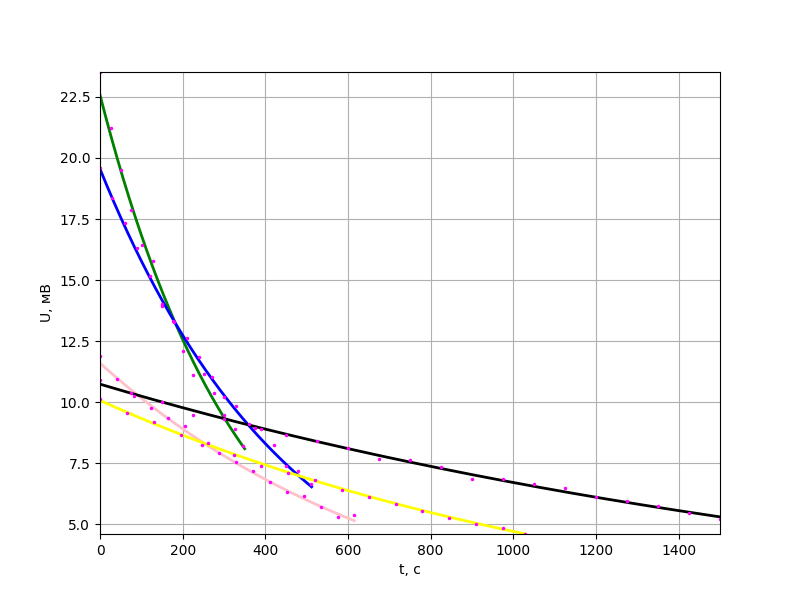
\includegraphics[scale=0.8]{Pictures/Все(эксп).png}
	\caption*{График 1. Экспоненциальная зависимость. Цвета: зеленый - 40 торр, синий - 60 торр, розовый - 90 торр, желтый - 140 торр, черный - 250 торр}
\end{figure}
\vspace{10mm}
\newpage
В логарифмическом масштабе получаем следующие графики:
\begin{figure}[h!]
	\centering
	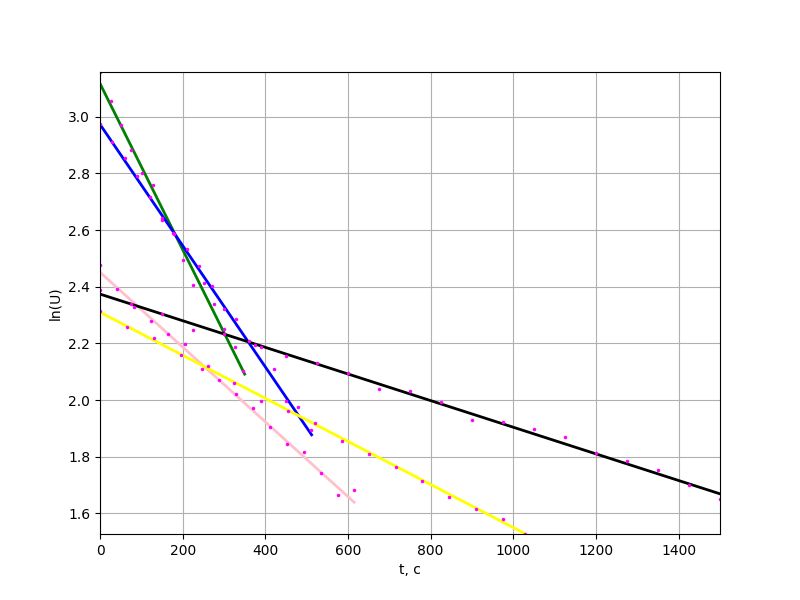
\includegraphics[scale=0.8]{Pictures/Все(лин).png}
	\caption*{График 2. Линейная зависимость. Цвета: зеленый - 40 торр, синий - 60 торр, розовый - 90 торр, желтый - 140 торр, черный - 250 торр}
\end{figure}

\item Убедимся, что процесс диффузии подчиняется закону (6). С этой целью для каждого из давлений построим графики, откладывая по оси абсцисс время, а по оси ординат — логарифм от показаний вольтметра. По угловым коэффициентам экспериментальных прямых и известным параметрам установки рассчитаем коэффициенты взаимной диффузии при выбранных давлениях.


1) $P = $ 40 торр.

Используя МНК, получаем такой график для экспоненциальной зависимости:
\newpage
\begin{figure}[h!]
	\centering
	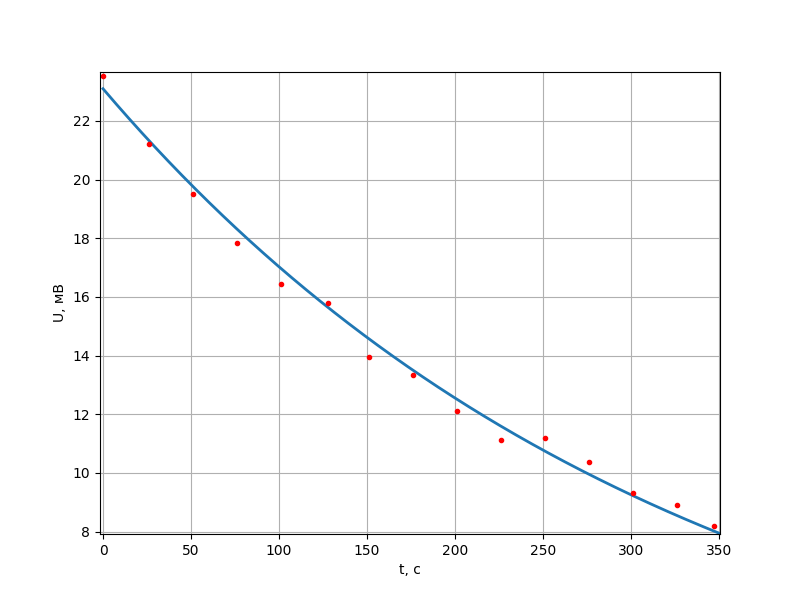
\includegraphics[scale=0.8]{Pictures/График1(эксп).png}
	\caption*{График 3}
\end{figure}

Теперь в логарифмическом масштабе:

$U(t) = U_{0}e^{-\frac{t}{\tau}}$,


где $\tau = \frac{V_{1}V_{2}}{V_{1} + V_{2}}\frac{l}{S}\frac{1}{D}$ - постоянная времени для данного давления. $V_{1} = (1200\pm 30)$ см$^{3}$ - объем сосуда с гелием, $V_{2} = (1200\pm 30)$ см$^{3}$ - объем сосуда с воздухом, $\frac{l}{S} = (5,5\pm 0,5)$ $\frac{1}{\text{см}}$, $D$ - коэффициент взаимной диффузии.  
	
	
$\ln{U} = \ln{U_{0}} - \frac{t}{\tau}$.

Используя МНК, получаем:

$k = -\frac{1}{\tau} = -0,00293$ c$^{-1}$

$\sigma_{k} = 6\cdot 10^{-5}$ c$^{-1}$

$D = \frac{V_{1}V_{2}}{V_{1} + V_{2}}\frac{l}{S}\frac{1}{\tau} = - \frac{V_{1}V_{2}}{V_{1} + V_{2}}\frac{l}{S}k$.

$D = $ 9,0 $\frac{\text{см}^2}{\text{c}}$
\newpage
\begin{figure}[h!]
	\centering
	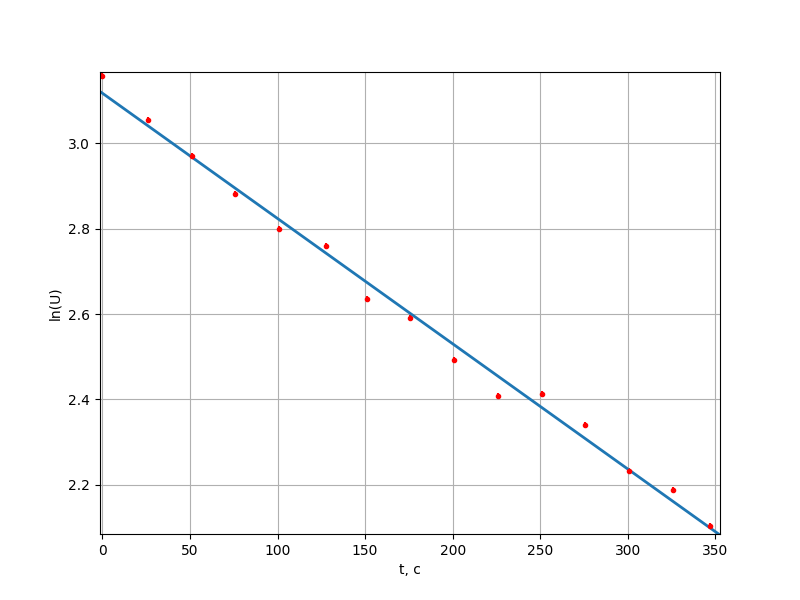
\includegraphics[scale=0.8]{Pictures/График1(лин).png}
	\caption*{График 4}
\end{figure}


$\sigma_{D} = D\sqrt{\left(\frac{\sigma_{V_{1}}}{V_{1}}\right)^2 + \left(\frac{\sigma_{V_{2}}}{V_{2}}\right)^2 + \left(\frac{\sigma_{V_{1} + V_{2}}}{V_{1}+V_{2}}\right)^2 + \left(\frac{\sigma_{\frac{l}{S}}}{\frac{l}{S}}\right)^2 + \left(\frac{\sigma_{k}}{k}\right)^2}$.

$\sigma_{V_{1} + V_{2}}^2 = \sigma_{V_{1}}^2 + \sigma_{V_{2}}^2$,

$\sigma_{D} = D\sqrt{\left(\frac{\sigma_{V_{1}}}{V_{1}}\right)^2 + \left(\frac{\sigma_{V_{2}}}{V_{2}}\right)^2 + \frac{\sigma_{V_{1}}^2 + \sigma_{V_{2}}^2}{(V_{1} + V_{2})^2} + \left(\frac{\sigma_{\frac{l}{S}}}{\frac{l}{S}}\right)^2 + \left(\frac{\sigma_{k}}{k}\right)^2}$.

$\sigma_{D} = $ 1,0 $\frac{\text{см}^2}{\text{c}}$.
\vspace{15mm}

$D = (9,0 \pm 1,0)$ $\frac{\text{см}^2}{\text{c}}$.

\newpage
2) $P = $ 60 торр.

Используя МНК, получаем такой график для экспоненциальной зависимости:
\begin{figure}[h!]
	\centering
	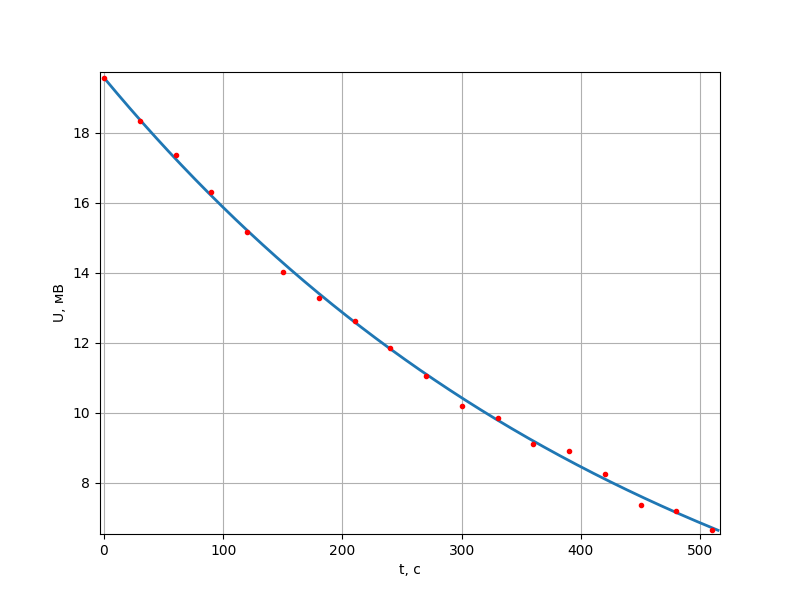
\includegraphics[scale=0.8]{Pictures/График2(эксп).png}
	\caption*{График 5}
\end{figure}

Теперь в логарифмическом масштабе:

$k = -\frac{1}{\tau} = -0,00214$ c$^{-1}$

$\sigma_{k} = 2\cdot 10^{-5}$ c$^{-1}$

$D = - \frac{V_{1}V_{2}}{V_{1} + V_{2}}\frac{l}{S}k$.

$D = $ 7,0 $\frac{\text{см}^2}{\text{c}}$

$\sigma_{D} = $ 0,7 $\frac{\text{см}^2}{\text{c}}$.
\vspace{15mm}

$D = (7,0 \pm 0,7)$ $\frac{\text{см}^2}{\text{c}}$.
\newpage
\begin{figure}[h!]
	\centering
	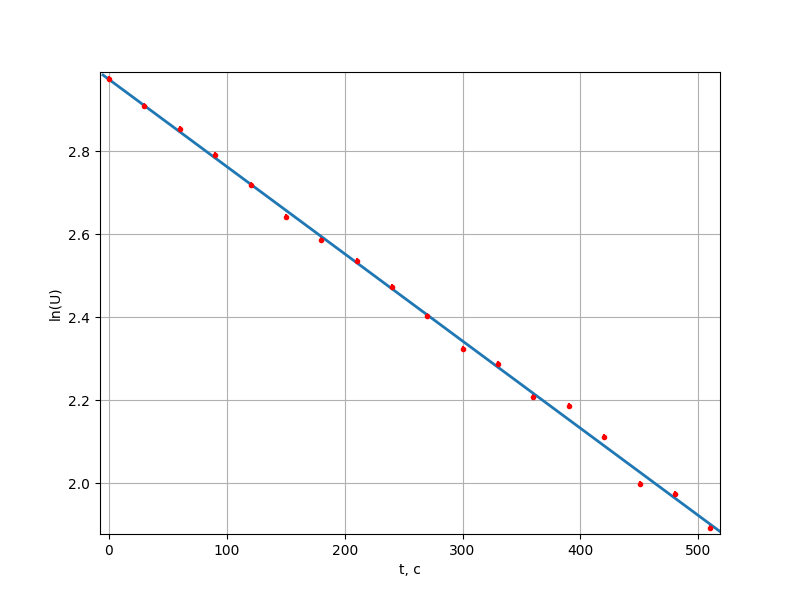
\includegraphics[scale=0.8]{Pictures/График2(лин).png}
	\caption*{График 6}
\end{figure}

\newpage

3) $P = $ 90 торр.

Используя МНК, получаем такой график для экспоненциальной зависимости:
\begin{figure}[h!]
	\centering
	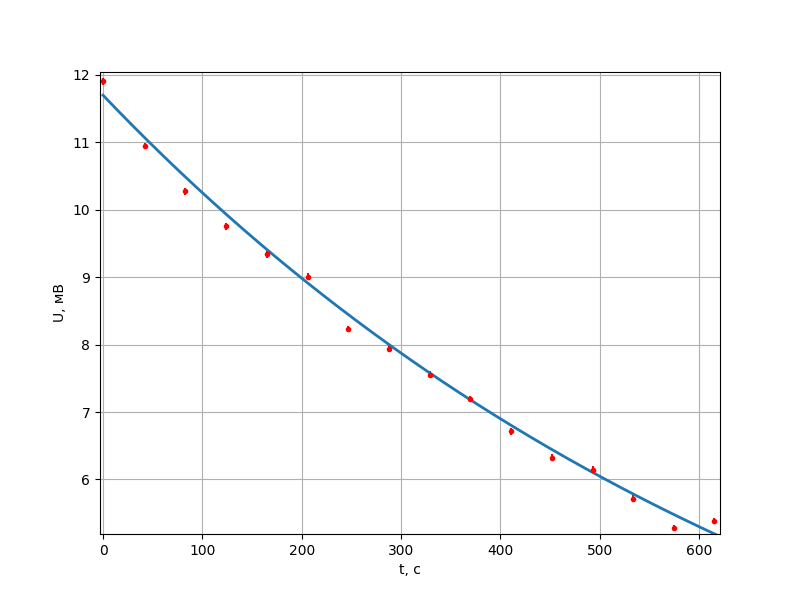
\includegraphics[scale=0.8]{Pictures/График3(эксп).png}
	\caption*{График 7}
\end{figure}

Теперь в логарифмическом масштабе:

$k = -\frac{1}{\tau} = -0,00132$ c$^{-1}$

$\sigma_{k} = 2\cdot 10^{-5}$ c$^{-1}$

$D = - \frac{V_{1}V_{2}}{V_{1} + V_{2}}\frac{l}{S}k$.

$D = $ 4,3 $\frac{\text{см}^2}{\text{c}}$

$\sigma_{D} = $ 0,5 $\frac{\text{см}^2}{\text{c}}$.
\vspace{15mm}

$D = (4,3 \pm 0,5)$ $\frac{\text{см}^2}{\text{c}}$.
\newpage
\begin{figure}[h!]
	\centering
	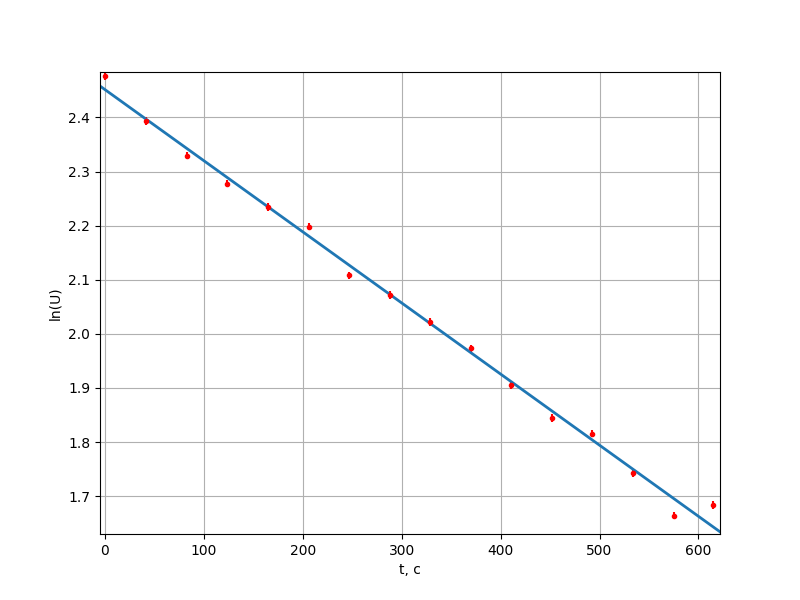
\includegraphics[scale=0.8]{Pictures/График3(лин).png}
	\caption*{График 8}
\end{figure}

\newpage

4) $P = $ 140 торр.

Используя МНК, получаем такой график для экспоненциальной зависимости:
\begin{figure}[h!]
	\centering
	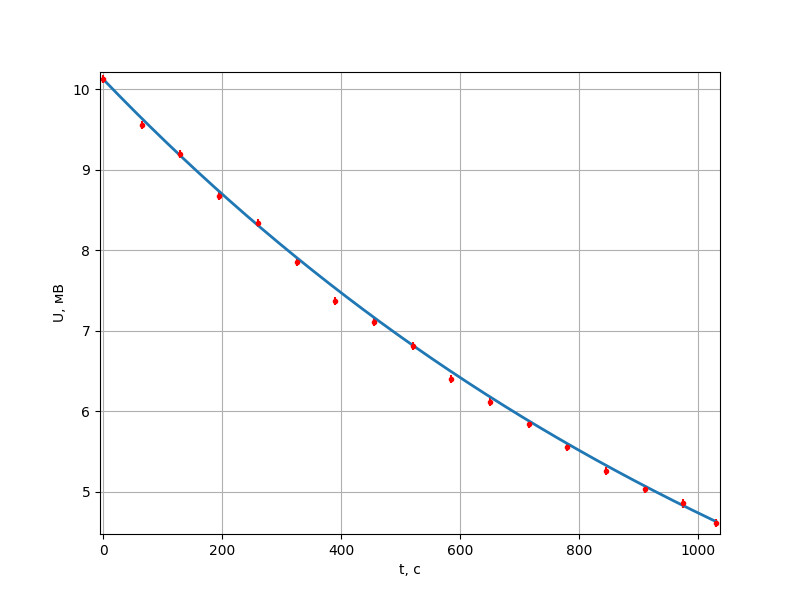
\includegraphics[scale=0.8]{Pictures/График4(эксп).png}
	\caption*{График 9}
\end{figure}

Теперь в логарифмическом масштабе:

$k = -\frac{1}{\tau} = -0,00076$ c$^{-1}$

$\sigma_{k} = 5\cdot 10^{-6}$ c$^{-1}$

$D = - \frac{V_{1}V_{2}}{V_{1} + V_{2}}\frac{l}{S}k$.

$D = $ 2,5 $\frac{\text{см}^2}{\text{c}}$

$\sigma_{D} = $ 0,3 $\frac{\text{см}^2}{\text{c}}$.
\vspace{15mm}

$D = (2,5 \pm 0,3)$ $\frac{\text{см}^2}{\text{c}}$.
\newpage
\begin{figure}[h!]
	\centering
	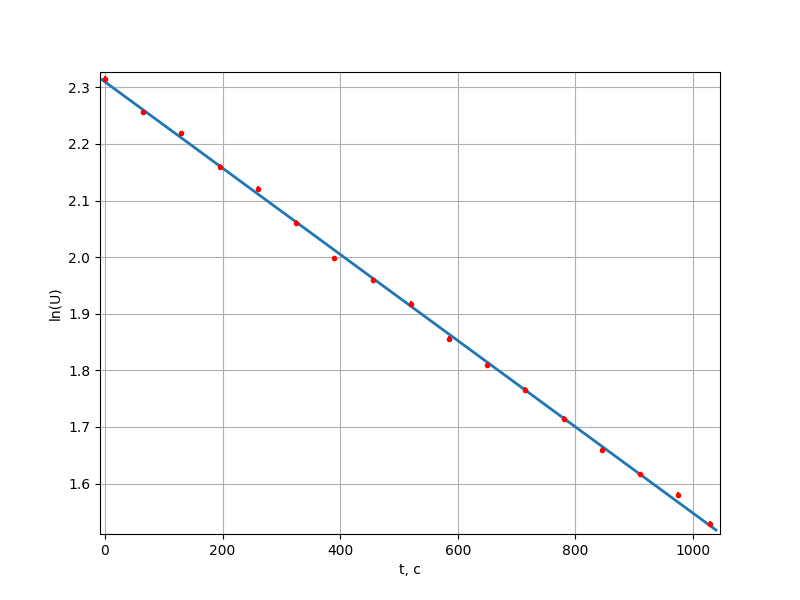
\includegraphics[scale=0.8]{Pictures/График4(лин).png}
	\caption*{График 10}
\end{figure}

\newpage


5) $P = $ 250 торр.

Используя МНК, получаем такой график для экспоненциальной зависимости:
\begin{figure}[h!]
	\centering
	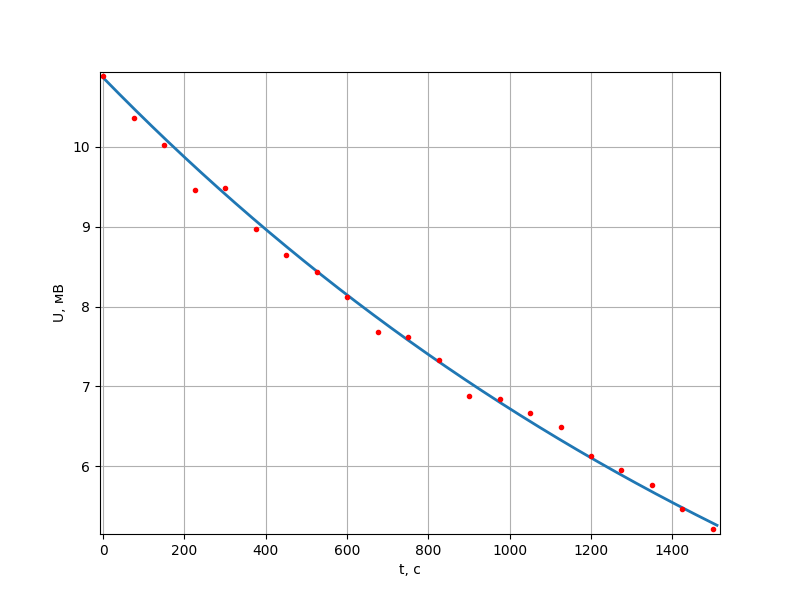
\includegraphics[scale=0.8]{Pictures/График5(эксп).png}
	\caption*{График 11}
\end{figure}

Теперь в логарифмическом масштабе:

$k = -\frac{1}{\tau} = -0,00047$ c$^{-1}$

$\sigma_{k} = 6\cdot 10^{-6}$ c$^{-1}$

$D = - \frac{V_{1}V_{2}}{V_{1} + V_{2}}\frac{l}{S}k$.

$D = $ 1,5 $\frac{\text{см}^2}{\text{c}}$

$\sigma_{D} = $ 0,2 $\frac{\text{см}^2}{\text{c}}$.
\vspace{15mm}

$D = (1,5 \pm 0,2)$ $\frac{\text{см}^2}{\text{c}}$.
\newpage
\begin{figure}[h!]
	\centering
	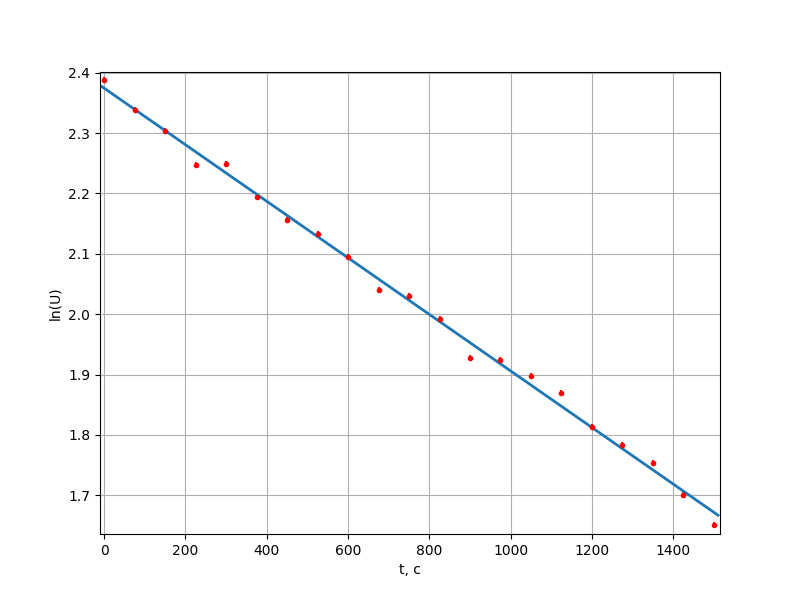
\includegraphics[scale=0.8]{Pictures/График5(лин).png}
	\caption*{График 12}
\end{figure}

\newpage

\item Построим график зависимости коэффициента диффузии от давления в координатах $D, 1/P$.

\begin{table}[h!]
	\centering
	\begin{tabular}{|c|l|l|l|}
		\hline
		$P$, торр & \multicolumn{1}{c|}{$\frac{1}{P}$,  $\text{торр}^{-1}$} & \multicolumn{1}{c|}{$D$, $\frac{\text{см}^2}{\text{c}}$} & \multicolumn{1}{c|}{$\sigma_{D}$, $\frac{\text{см}^2}{\text{с}}$} \\ \hline
		40        & 0,0250                                                  & 9,0                                                      & 1,0                                                               \\ \hline
		60        & 0,0167                                                  & 7,0                                                      & 0,7                                                               \\ \hline
		90        & 0,0111                                                  & 4,3                                                      & 0,5                                                               \\ \hline
		140       & 0,0071                                                  & 2,5                                                      & 0,3                                                               \\ \hline
		250       & 0,0040                                                  & 1,5                                                      & 0,2                                                               \\ \hline
	\end{tabular}
\caption*{Таблица 6}
\end{table}

Погрешности $D$ известны, поэтому используем метод $\chi^2$.


$D = k\cdot \frac{1}{P}$.

\begin{figure}[h!]
	\centering
	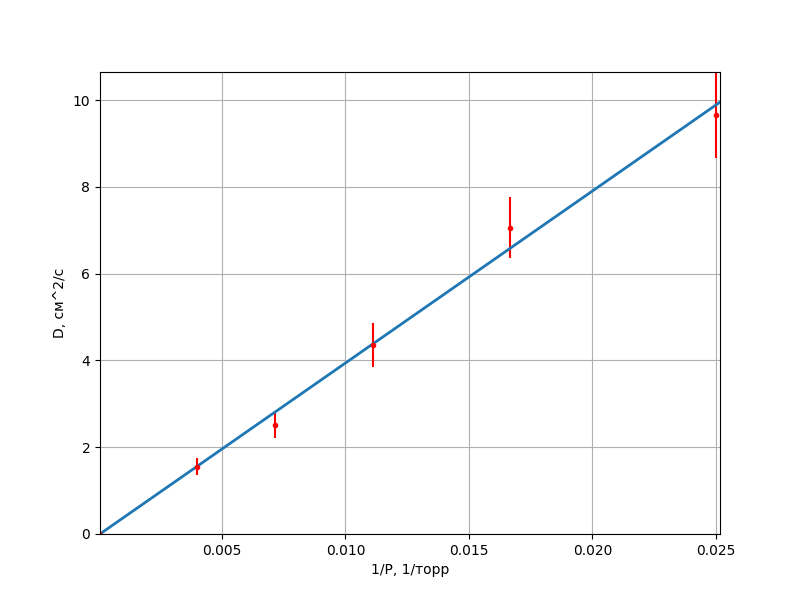
\includegraphics[scale=0.8]{Pictures/D(P).png}
	\caption*{График 13}
\end{figure}

\newpage

Получаем:

$k = 413$ $\frac{\text{см}^2}{\text{c}\cdot\text{торр}}$.

$\sigma_{k} = 42$ $\frac{\text{см}^2}{\text{c}\cdot\text{торр}}$.

$k = (413 \pm 42)$ $\frac{\text{см}^2}{\text{c}\cdot\text{торр}}$.

\vspace{10mm}

Значение $\chi^2 = $ 2,3.

\vspace{15mm}

Рассчитаем величину коэффициента диффузии при атмосферном давлении, т.е. при 760 торр. 


Лучшая прямая:

$D = 413\cdot \frac{1}{P}$

$D_{\text{атм}} = \frac{413}{760}$ $\frac{\text{см}^2}{\text{c}}$ = $0,54$ $\frac{\text{см}^2}{\text{c}}$.

$\sigma_{D_{\text{атм}}} = D_{\text{атм}} \cdot \frac{\sigma_{k}}{k} = 0,54 \cdot \frac{42}{413}$ $\frac{\text{см}^2}{\text{c}}$ = $0,06$ $\frac{\text{см}^2}{\text{c}}$.


$D_{\text{атм}} = (0,54\pm 0,06)$ $\frac{\text{см}^2}{\text{c}}$.

Данное значение достаточно близко к табличному. Оно отличается от последнего на $\thicksim$ 11\%.


\item Оценим по полученным результатам длину свободного пробега и размер атома гелия.


$D = \frac{1}{3}\lambda\bar{v}$

$\lambda = \frac{3D}{\bar{v}} \thicksim \frac{3D\sqrt{\pi\mu_{\text{He}}}}{\sqrt{8RT}} \thicksim 1,5\cdot 10^{-7}$ м

$\lambda = \frac{1}{\sqrt{2}n\sigma} = \frac{kT}{\sqrt{2}p\pi d^2}$


$d = \sqrt{\frac{kT}{\sqrt{2}p\pi\lambda}} \thicksim 2,5\cdot 10^{-10}$ м


Данные значения немало отличаются от табличных, однако они хотя бы имеют тот же порядок:

$\lambda_{\text{табл}} \approx 1,8\cdot 10^{-7}$ м \hspace{60mm} $d_{\text{табл}} \approx 2\cdot 10^{-10}$ м.
\end{enumerate}

\newpage

\section*{Вывод}
В работе была проведена регистрация зависимости концентрации гелия в воздухе от времени с помощью датчиков теплопроводности при разных начальных давлениях смеси газов. Также был определен коэффициента взаимной диффузии гелий - воздух при атмосферном давлении: $D = (0,54\pm 0,06)$ $\frac{\text{см}^2}{\text{c}}$. Помимо этого по полученным данным были оценены средняя длина свободного пробега и диаметр атомов гелия: $\lambda \thicksim 1,5\cdot 10^{-7}$ м, $d \thicksim 2,5\cdot 10^{-10}$ м. Оценка этих величин достаточно посредственная, однако их порядки совпадают с порядками табличных значений. Ошибки связаны с неточностью измерений и несовершенством техники измерения.
\end{document}